\begin{savequote}[75mm]
[A computer] takes these very simple-minded instructions -- 'go fetch a number, add it to this number, put the result there, perceive if it's greater than this other number' -- but executes them at a rate of, let's say, 1,000,000 per second. At 1,000,000 per second, the results are indistinguishable from magic.
\qauthor{Steve Jobs (1955-2011)}
\end{savequote}

\chapter{Locating Optimal Corridors}
\label{Chapter 2}

\newpage

  \section{Locating Optimal Corridors for Water Distribution Infrastructure}
 
\newthought{The source of location} for the delivery of treated wastewater for artificial groundwater recharge applications is always the Wastewater Treatment Plant (WWTP). WWTPs are overwhelming located at low elevation points within the hydrological basins that they serve; as this feature ensures a minimum energy input requirement to deliver wastewater from its distributed sites of generation (i.e. the many homes and businesses distributed geographically throughout the basin) to a single centralized point of treatment. In this way, a system design based upon a single centralized WWTP is best able to take advantage of the use of gravity to provide the motive force for the wastewater's journey through the system. As a side note, an question which may become of substantial future interest is how a more prominent role of reuse may alter our thinking about the optimal design of water treatment collection and conveyance infrastructure. Specifically, it remains an open research question as to whether or not the existing paradigm, with large centrally location treatment facilities, would persist as the most favorable solution if one were charged with designing an integrated wastewater treatment and reuse system from the oft.
                
The salient output of the first model component - WOSS - is the designation of one or more suitable sites for the placement of either a gravity fed surface spreading infiltration basin or a pump driven subsurface recharge well. In this way, we are left with one or many (in the case of multiple suitable sites) combinations of point source and destination locations. The next modeling challenge which must be overcome therefore is the development of a scheme for generating plausible pathways which connect the source locations to the various destinations. The implicit assumption here being, that in order to deliver the treated wastewater from its source of production, the WWTP, to the end point of use, the recharge site, new water conveyance infrastructure must be constructed.
        
At this stage it is important to pause to consider whether or not the construction of new water conveyance infrastructure is in fact a necessary condition of all or any water reuse projects. There are two perspectives from which a response to this objection can be framed. The first is technical in nature. If no new conveyance structure is implemented, two fundamental technical requirements must be met. The first is that the point of reuse must be situated favorably with respect to the existing potable water conveyance system such that it can be readily be connected to, and withdraw from it, large quantities of water for recharge purposes. The second is that the treated wastewater which is to be reused must be returned to a sufficiently high standard of quality such that it can be reincorporated directly back into the potable water supply. This second constraint, while technically feasible given sufficient financial resources, leads naturally to the other category of potential objections to the development of a reuse project without the addition of new conveyance infrastructure: namely, the social stigma associated with co-mingling so-called reclaimed "black water," with the potable freshwater supply. There is a considerable body of research in the social sciences which suggests that a majority of people harbor a very basic, if somewhat irrational, prejudice against the direct reuse of reclaimed water for potable applications. 
            
\section{The Multi-Objective Corridor Location Problem}
            
The multi-objective corridor location problem can be formally written as Equation 1 \cite{Zhou2011}. The problem involves the simultaneous minimization of the sums of $w$ independent objective functions $\hat{O}_w$ evaluated at the set of discrete locations $\textbf{x}_n$ comprising a corridor of length $n$. A valid corridor $\textbf{x}_n$ is subject to the constraint that all of its nodes must be contained with the feasible search domain $\boldsymbol{\Omega}$. Additional, optional constraints which are often imposed upon the structure of $\textbf{x}_n$ shall be discussed in greater detail in subsequent sections.
            
            \begin{equation}
            Minimize: \prod\limits_{n=1}^n \left\{\hat{O}_1(\textbf{x}_n), \dots, \hat{O}_w(\textbf{x}_n)\right\} 
            \end{equation}
            \begin{equation}
            S.t.: \textbf{x}_n \in \boldsymbol\Omega
            \end{equation}
            
            \noindent \textit{Where:} \hfill
            
            \begin{center}
            $\textbf{x}_n =$ The set of discrete row column indices defining a corridor of length $n$
            \\
            $\boldsymbol{\Omega} =$ The set of discrete row column indices defining the feasible decision space
            \\
            $O_w =$ The true but unknown forms of $w$ continuous objective functions
            \\
            $\hat{O}_w =$ The estimates of $O_w$ defined over the discrete set $\boldsymbol{\Omega}$
            \end{center}
                        
As a subset of SPPs, corridor location problems tend to be defined in the context of networks with large numbers of nodes and highly structured topologies \cite{Goodchild1977}. These shared characteristics arise from the fact that corridor location problems are typically posed in the context of continuous geographic space – a feature which requires that the requisite underlying network structure be generated algorithmically \cite{Stefanakis1995}. In practice, this is frequently accomplished by automating the conversion of a geographically referenced raster grid into a set of nodes by referencing the the centroids of the cells within the raster in a process similar to that described by \cite{Huber1985}. Once the nodes in the network have been created they can then connected to one another by automatically generating arcs using some standard mode of node connectivity; again, using methods similar to those described by \cite{Church1992}.
            
\section{Genetic Algorithms}

Genetic Algorithms (GAs) are a family of search heuristics that mimic the process of natural selection to derive one or more near optimal solutions to a given optimization problem. \cite{Goldberg1989} GAs constitute a subset of Evolutionary Algorithms (EAs) which encode solutions using data structures that are analogous to biological chromosomes \cite{Deb2001}. This feature allows the search for new, better solutions to be accomplished via the iterative application of genetic operations such as crossover, mutation, selection, etc. \cite{Goldberg1988} GAs have been developed and profitably used in a wide variety of problem domains from engineering and economics to chemistry and physics. General purpose reviews of the application of GAs to various problems are available from the following references. \cite{Fonseca1995, Zitzler1998, Coello2001} For a more specialized reviews regarding state of the art applications of multi-objective genetic algorithms see the excellent book from Coello \& Lamont and, more recently, from Zhou \textit{et al}. \cite{Coello2007, Zhou2011}
            
\section{The MOGADOR Algorithm}
            
MOGADOR is an acronym stands for “Multiple Objective Genetic Algorithm for Corridor Selection Problems.” \cite{Zhang2008} The algorithm was introduced as a novel genetic approach to the problem of multi-objective corridor search. \cite{Mooney2006, Zhang2008} It development was intended to service need for a robust method of siting optimal corridors relevant to a variety of environmental planning and design applications. \cite{Bennett2004, Chakhar2003, Zhou1996} A need which persisted despite numerous previous efforts to adapt general purpose, deterministic, SSP solution techniques for use in corridor location. \cite{Hallam2001, Jankowski1995, Lombard1993} The continued need for refined algorithmic approaches to the location of optimal corridors within a broad range of application domains is evidenced by the continued appearance of closely related publications during the intervening years. \cite{Aissi2012, Mousseau2010, Neema2010, Roberts2010, Scaparra2014, Tsai2011} 

Relative to other traditional shortest path finding routines, the MOGADOR algorithm has been observed to possess a number of favorable characteristics. First among these is the ability of MOGADOR to accommodate large problem statements (large $\boldsymbol{\Omega}$) and or those which require the simultaneous evaluation of large numbers of independent objectives (large $w$) (Pangilinan \& Janssens 2007, Zhang et al 2008). Another useful feature of the MOGADOR algorithm is its ability to generate an entire solution set from a single run – as opposed to the single solution per run which is typical of traditional SPP algorithms (Cherkassky et al 1996, Dreyfus 1969, Hart et al 1968, Zhang et al 2008). Lastly, but perhaps most importantly, is that when properly parameterized, each of the solutions generated by the MOGADOR algorithm can be said to be non-inferior to every other (Zhang et al 2008). In this way, the output solution set approximates the so called Pareto optimal solution set for the given problem statement (Deb 2014).  

In order to proceed with our discussion of the MOGADOR algorithm, some basic terminology must first be defined. In the context of the MOGADOR algorithm a single gene $\textbf{x}$ is comprised of a pair of row column indices $(r,c)$ to a geographically referenced 2-D array comprising the feasible search domain $\boldsymbol{\Omega}$. An individual $\textbf{I}_m$ is comprised of a sequence of row column index vectors $\textbf{x}_n$ which collectively form a valid pathway between a predefined set of source ${}^{s}\textbf{x}$ and destination ${}^{d}\textbf{x}$ locations. In this way, each individual represents a feasible solution to the proposed corridor location problem. A population $\textbf{P}_g$ is comprised of $m$ individuals. And, finally, an evolution $\textbf{E}_b$ is comprised of $g$ populations.

Figure 1 provides a pseudocode description of the MOGADOR algorithm. Its structural components are fairly typical among GAs in general. The search process begins with a stochastic routine for generating of an initial seed population $\textbf{P}_1$. Following the initialization of this seed population, the fitness $\textbf{F}_1$ of each individual in the seed population is computed by summing the objective function scores corresponding to each set of nodes comprising each individual. Upon the completion of this initialization phase, the algorithm then enters a loop wherein successive genetic operations are applied to the initial seed population. In the case of MOGADOR, these operators include: the selection individuals for reproduction on the based upon their fitness, the crossover of selected individuals that share at least one common feature, and finally, the mutation of crossed over individuals so as to maintain a degree of random variation within the population. At the end of each loop iteration a new population is generated, its fitness evaluated, and a convergence parameter computed on the basis of the observed rate of improvement in population fitness across previous iterations. If convergence is achieved $(c_g < {}^{t}c)$ the loop is broken and the algorithm terminates returning: the evolutionary history of the population $\textbf{P}_{1:g}$, the corresponding fitness values each individual within the population $\textbf{F}_{1:g}$, and the convergence parameter history $\textbf{C}_{1:g}$. \\

                \begin{algorithm}
                \caption{}\label{euclid}
                \begin{algorithmic}[1]
                \Procedure{MOGADOR}{}
                \State $g = 1 \gets$ initialize loop iterator
                \State $c_g = 0 \gets$ initialize convergence parameter
                \State \textbf{P}$_g = initializeSeedPopulation(m,\boldsymbol\Omega)$
                \State \textbf{F}$_g = computePopulationFitness($\textbf{P}$_g,\hat{O}_w)$ 
                \While{$c_g < $ \textsuperscript{\textit{t}}$c$}{}:
                \State $g += 1 \gets$ update loop iterator
                \State \textbf{S}$_g = selectIndividualsFromPopulation($\textbf{P}$_g)$
                \State \textbf{X}$_g = crossoverSelectedIndividuals($\textbf{S}$_g)$
                \State \textbf{P}$_g = mutateCrossoverIndividuals($\textbf{X}$_g)$
                \State \textbf{F}$_g = computePopulationFitness($\textbf{P}$_g)$
                \State $c_g = computeConvergenceParameter($\textbf{F}$_{1:g})$
                \State \textbf{end}
                \EndWhile
                \State \textbf{return: \textbf{P}$_{1:g},$ \textbf{F}$_{1:g},$ \textbf{C}$_{1:g}$}
                \EndProcedure
                \end{algorithmic}
                \end{algorithm}
                
            \begin{figure}[MOGADOR Algorithm Pseudocode]
            \caption[MOGADOR Algorithm Pseudocode]{MOGADOR Algorithm Pseudocode}
            \label{fig:mogador-pseudocode}
            \end{figure}
    
\section{The MOGADOR Data Structure}
    
The optimal data structure for use in concert with the MOGADOR algorithm is a nested list of lists. Such a list based data structure is well suited to this context as there can be a high degree of variability in the number of elements produced by the different stochastic genetic operators.1 Figure 2 illustrates a small but valid example such a nested list of lists data structure as used in the context of the MOGADOR algorithm. Note, for example, how the number of row column index vectors $n$ in the first individual $\textbf{I}_1$ equals 5, while the number of index vectors in subsequent individuals $\textbf{I}_{2:4}$ belonging to the same population, ranges between 3 and 6. The source of this variation has to do with the stochasticity inherent to the population initialization routine. Similarly, note how the number of populations $g$ in the first evolution $\textbf{E}_1$ is 3 while the number of populations in the second evolution is 4. The source of this variation has to do with the stochasticity in the crossover and mutation processes. Indeed, the only level of the data structure's hierarchy at which a constant number of elements is required is at the population level. Meaning, in other words, that each population $\textbf{P}_g$ contained within evolutions $\textbf{E}_b$ must all possess the same number of $m$ individuals. This requirement ensures that the behavior of the genetic operators is consistent between separate evolutions.
            
            \begin{figure}[MOGADOR Algorithm Data Structure]
            \centering
            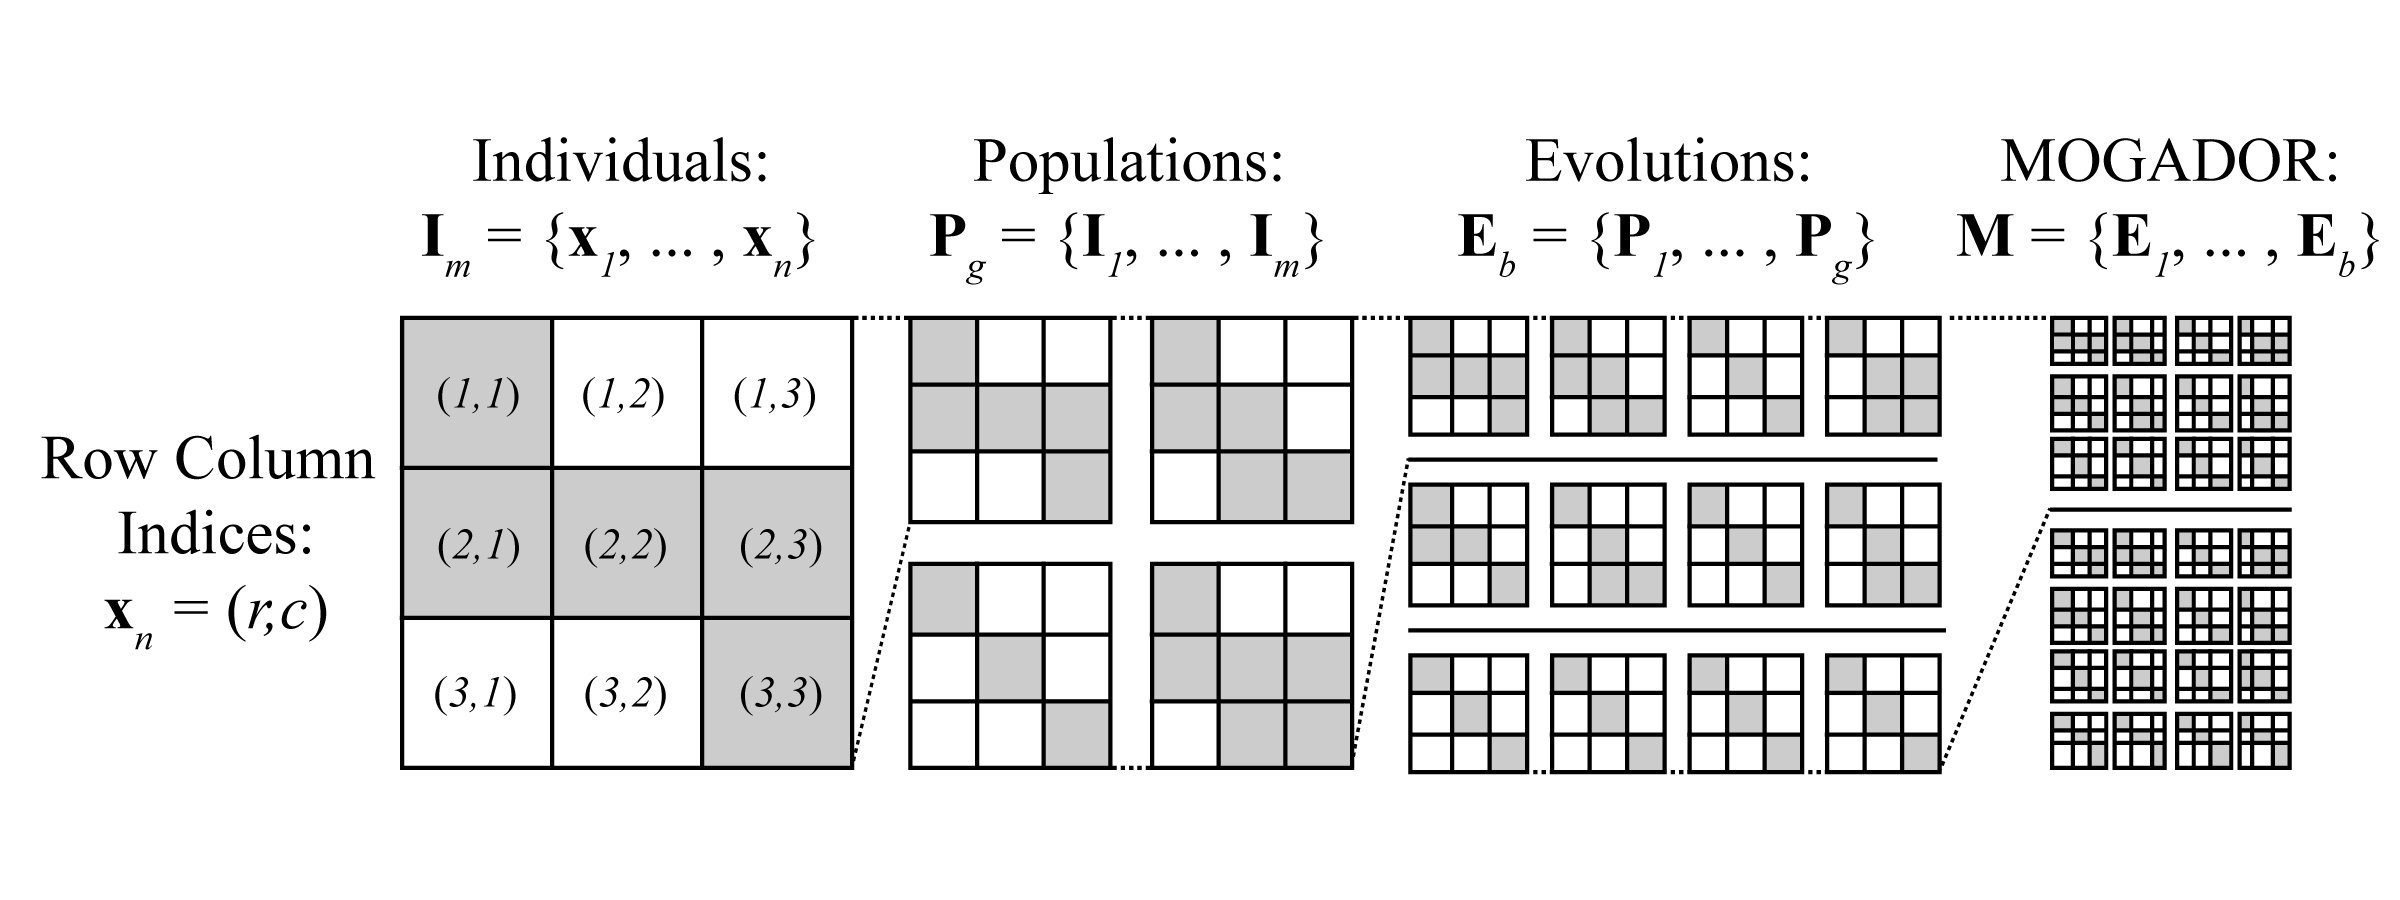
\includegraphics[width=5.5in]{figures/data-structure.png}   
            \caption[MOGADOR Algorithm Data Structure]{MOGADOR Algorithm Data Structure}
            \label{fig:data-structure}
            \end{figure}

\section{Initializing the MOGADOR Algorithm}
    
A novel population initialization procedure has been developed for use in conjunction with the MOGADOR algorithm which improves the global quality of the output solution set while simultaneously reducing overall computational effort. At its core, this novel pseudo-random walk algorithm works by repeatedly sampling a dynamically parameterized bivariate Gaussian distribution. The generic form of the probability density function for the bivariate Gaussian distribution can be written as Equation 2 (Johnson et al 2002). Here, the bivariate Gaussian PDF $f(\boldsymbol{\tau})$ is function of two inputs. [1] The first is a mean vector $\boldsymbol{\mu}$, comprised of the means $(\mu_1, \mu_2)$ of two continuous random variables $(\tau_1, \tau_2)$. [2] The second is a covariance matrix $\boldsymbol{\Sigma}$, comprised of the pairwise covariances $\sigma$ for all possible combinations of the continuous random variables $(\tau_1, \tau_2)$.
            
            \begin{equation}
            f(\boldsymbol{\tau}) = \frac{1}{ \sqrt{ (2\pi)^2 \mid \boldsymbol{\Sigma} \mid} } e^{ \frac{-1}{2} ( \boldsymbol{\tau} - \boldsymbol{\mu} )^T \boldsymbol{ \Sigma}^{-1} ( \boldsymbol{\tau} - \boldsymbol{\mu} ) }
            \end{equation}

            \noindent \textit{Where:} \hfill

            \begin{center}
            $\boldsymbol{\tau} =$ The set of correlated continuous random variables $(\tau_1, \tau_2)$
            \\
            $\boldsymbol{\mu} = $ The set of mean values $(\mu_1, \mu_2)$ for $(\tau_1, \tau_2)$
            \\
            $\boldsymbol{\Sigma} =$ The pairwise covariance structure $\bigl[\begin{smallmatrix} \sigma(\tau_{1},\tau_{1}) & \sigma(\tau_{1},\tau_{2}) \\ \sigma(\tau_{2},\tau_{1}) & \sigma(\tau_{2},\tau_{2}) \\ \end{smallmatrix}\bigr]$ for $(\tau_{1}, \tau_{2})$
            \end{center}
            
Each sampled value for $\tau_1, \tau_2$ can be reduced to a unit vector and interpreted as a set of row column index deltas. The repeated sampling of the distribution therefore provides a simple yet powerful technique for generating randomized positional changes within a 2-D lattice. Additionally, as shall be discussed in the subsequent sections, the ability to dynamically adjust the parameters of the bivariate Gaussian PDF at any time during the sampling process provides a mechanism by which one is able to functionally constrain the randomness of the walk; hence the term: pseudo-random walk.
            
Figure 3 provides a pseudocode representation of the proposed pseudo-random walk procedure. Structurally, the routine consists of two nested while loops. At each iteration $h$ of the outer loop a single step $\textbf{x}_n$ along an individual walk $\textbf{I}_m$ is taken. This loop continues until the location of the current step is equal to that of the destination ${}^{d}\textbf{x}$. At each iteration $u$ of the inner loop a candidate next step $\Delta \textbf{x}_u$ is produced by random sampling the parameterized bivariate Gaussian PDF $f(\textbf{x}_u)$. Candidate next steps are only considered valid if they are contained within the current valid connected set $\textbf{V}_n$. The current valid connected set is comprised of all neighboring nodes that not been previously visited and that are inclusive to the search domain $\boldsymbol{\Omega}$.  If the candidate step is found to be valid the inner loop terminates, the outer loop iterates, and the walk process continues. If the valid set is ever found to be empty the outer loop iterator $h$ is reset and the entire process is restarted. \\
            
                \begin{algorithm}
                \caption{}\label{euclid}
                \begin{algorithmic}[1]
                \Procedure{PSEUDO-RANDOM WALK}{}
                \State $n = 1 \gets$ initialize outer loop iterator
                \State $\textbf{x}_n =$ \textsuperscript{\textit{s}}$\textbf{x} \gets$ initialize individual at source
                \State \textbf{I}$^{*} = computeEuclideanShortestPath($\textsuperscript{\textit{s}}$\textbf{\textit{x}},$\textsuperscript{\textit{d}}$\textbf{x})$
                \While{$\textbf{x}_n \neq$ \textsuperscript{\textit{d}}$\textbf{x}$}{}:
                \State $\textbf{V}_n = computeValidConnectedSet(\textbf{x}_{1:n},\boldsymbol\Omega)$
                \If{$\textbf{V}_n = \emptyset$}:
                \State $n = 1 \gets$ reset outer loop iterator
                \State \textbf{continue}
                \EndIf
                \State $u = 1 \gets$ initialize inner loop iterator
                \State $\boldsymbol{\mu}_n = computeOrientationVector(\textbf{x}_n,$\textsuperscript{\textit{d}}$\textbf{x})$
                \State $d_n = computeMinimumBasisDistance(\textbf{x}_{n},\textbf{I}^{*})$
                \State $n = n + 1 \gets$ update outer loop iterator
                \While{$\textbf{x}_n \not \in \textbf{V}_n$}{}:
                \State $\Sigma_u = computeCovarianceMatrix(d_n,u)$
                \State $\Delta\textbf{x}_u = sampleBivariateGaussianDistribution(\boldsymbol\mu_n,\Sigma_u)$
                \State $\textbf{x}_{n} = \textbf{x}_{n-1} + \Delta\textbf{x}_{u}$
                \State $u = u + 1 \gets$ update inner loop iterator
                \EndWhile {}
                \EndWhile {}
                \State \textbf{return: $\textbf{x}_{1:n}$}
                \EndProcedure
                \end{algorithmic}
                \end{algorithm}
                
            \begin{figure}[Pseudo-Random Walk Algorithm Pseudocode]
            \caption[Pseudo-Random Walk Algorithm Pseudocode]{Pseudo-Random Walk Algorithm Pseudocode}
            \label{fig:pseudo-random-walk-pseudocode}
            \end{figure}
            
In the process of sampling the parameterized bivariate Gaussian distribution the following three pieces of information are used to functionally constrain the probabilities associated with each candidate next step $\Delta\textbf{x}_u$. [1] At the start of each walk the set of array indices corresponding to the Euclidean shortest path $\textbf{I}^*$ from the source to the destination are generated using Bresenham's line algorithm (Bresenham 1977). Using this set of indices the minimum distance $d_n$ from the current position to the nearest point along this Euclidean shortest path is determined. [2] Next, at each step an orientation vector is computed indicating the orientation of the destination location relative to the current position. [3] Finally, each time the bivariate Gaussian PDF is sampled a counter variable $u$ is iterated. 

The orientation vector is interpreted as the mean of the bivariate Gaussian $PDF(\mu_n)$. Alternatively, the minimum distance and iteration variables $(d_n ,u)$ are processed as inputs to a generator function which produces the covariance matrix $\boldsymbol{\Sigma}_u$. This composition of this generator function ensures that the degree of randomness inherent to the selection of each next step is directly related to number of iterations while at the same time being inversely related to the minimum distance from the current location to the Euclidean shortest path.
            
\section{An Example Pseudo-Random Walk}

In an effort to make this pseudo-random walk procedure more comprehensible, particularly with regards to the parameterization of the bivariate Gaussian PDF $f(\textbf{x}_u)$, an example implementation is provided in Figure 4. On the far left of Figure 4 the current status of an arbitrary pseudo-random walk is shown midway through completion. Also drawn, as a broken line, is an abstract representation of the Euclidean shortest path $\textbf{I}^*$ connecting the source location ${}^{s}x$ to the destination location ${}^{d}x$. Show at bottom is the current value of the distance parameter $d_n \approx 7.1$. Just to the right of this, in the zoom inset area, the current valid connected set $\textbf{V}_n$ is drawn with the previously visited indices $(\textbf{x}_n ,\textbf{x}_{n-1})$ greyed out to illustrate their elimination from consideration as valid next steps in the walk process. Also shown in this inset are the row column unit vector deltas $\Delta\textbf{x}_u$ associated with movement to each of the seven nodes contained within the current valid connected set. The small arrow pointing downwards and to the right depicts the current state of the orientation vector $\boldsymbol\mu_n$ which describes the position of the destination location ${}^{d}\textbf{x}$ relative to the current walk location $\textbf{x}_n$. The current value of this vector $(\boldsymbol\mu_n = [1,1])$ can be thought of as indicating the row and column deltas associated the next step possible step most directly leading towards the destination.
            
            \begin{figure}[!h]
            \centering
            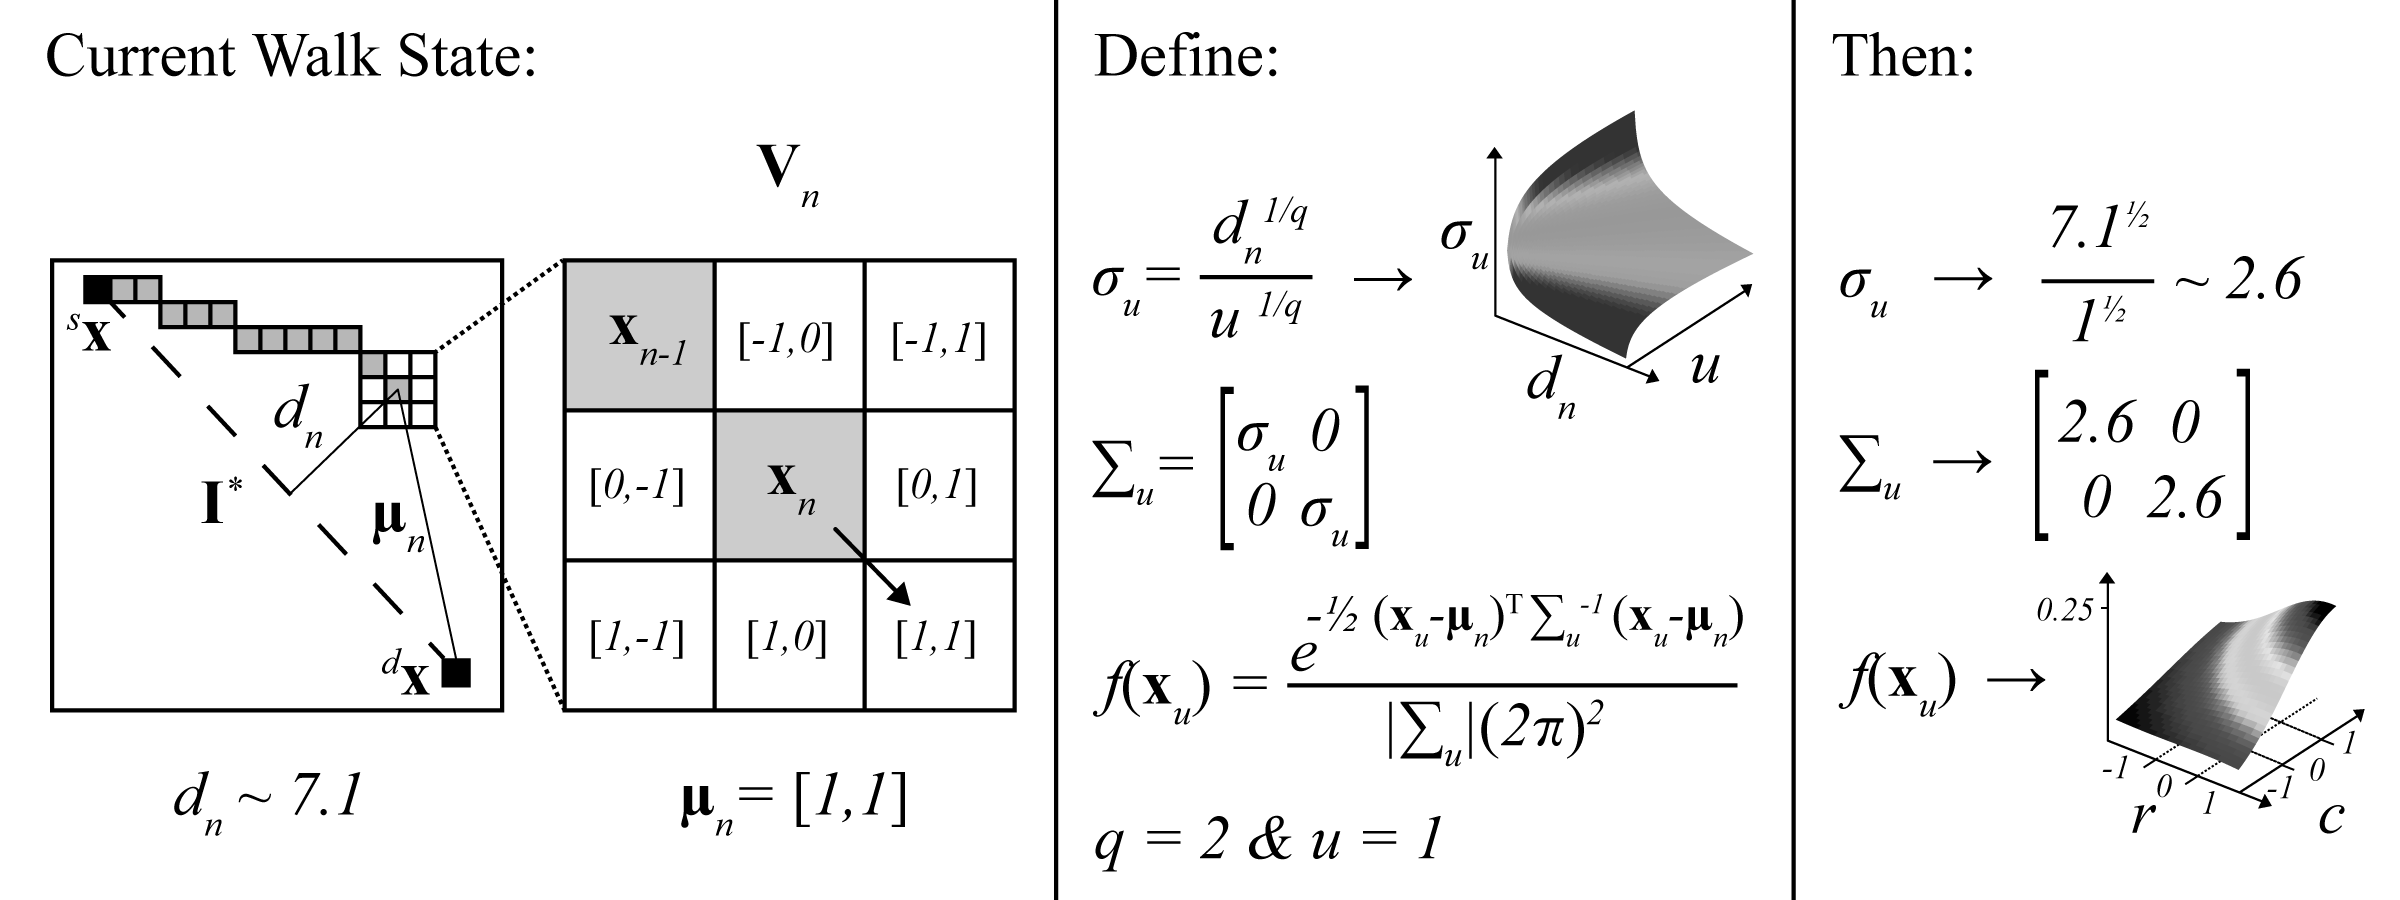
\includegraphics[width=5.5in]{figures/pseudo-random-walk-example.png}
            \caption[Pseudo-Random Walk Example]{Pseudo-Random Walk Example}
            \label{fig:pseudo-random-walk-example}
            \end{figure}
            
Continuing on to the right within Figure 4, three functions and two parameter values are defined. [1] First, the covariance term $\sigma_u$ for the current sample iteration $u$ is specified using a covariance generator function whose form enforces the relationship between distance, iteration count, and covariance previously described. A small demonstration plot of this function's form is provided. [2] Next, the covariance matrix $\boldsymbol\Sigma_u$ is defined by inserting the covariance term $\sigma_u$ to the diagonal elements of an empty square 2-D matrix. This repeated use of the same covariance term guarantees that for any value of $\sigma_u$ the output covariance matrix $\boldsymbol\Sigma_u$ will be positive definite. A square, symmetric, and positive definite covariance matrix is a hard requirement for the evaluation of the parameterized bivariate Gaussian PDF $f(\textbf{x}_u)$. The final two variable definitions $(q,u)$ are provided for the sake of computing illustrative values for the other parameters. Numerical evaluations of these expressions are given on the far right portion of the figure. Here again, a small demonstration plot showing the form of the evaluated bivariate Gaussian PDF $f(\textbf{x}_u)$ is provided.

One aspect of this process which warrants further discussion is the role of the fixed parameter $q$ in determining the degree of randomness exhibited by a given pseudo-random walk. The degree of randomness can be quantitatively defined as the range and extent to which the bivariate Gaussian PDF $f(\textbf{x}_u)$ deviates from its uniform bivariate counterpart. To illustrate this concept consider for example the characteristics of the PDF that would be required to produce a simple random walk using a similarly structured procedure. In such a case the value of $f(\textbf{x}_u)$ would have to be equal for all possible values of $\Delta\textbf{x}_u$. Due to the way in which the covariance generator function has been proposed, the $q$ parameter can therefore be used to determine the maximum range of variation in $\sigma_u$ which can be produced from any combination of $(d_n,u)$ input values. In this way, $q$ does not alter the structure of the bivariate Gaussian PDF $f(\textbf{x}_u)$ but rather only its magnitude. As a result, while the value of $q$ must always be greater than zero to produce real outputs from the covariance generator function, its value is inversely related to the degree of walk randomness. 

\section{Initializing Problems with Large Decisions Spaces}
    
While the pseudo-random walk procedure can be used to generate an initial seed population for any MOGADOR problem statement; a number of circumstances have been identified in which the performance of the population initialization procedure can be further refined. [1] The first such situation involves problems with extremely large decision spaces – defined as being thousands grid cells or more on a side. [2] The second problem specifications where it is known, a-priori, that the Euclidean path connecting the source to the destination is not entirely feasible.
            
Historically, corridor location problems which have been posed in the context of extremely large decisions spaces (large Ω) have been considered infeasible both for conventional deterministic SPP optimization techniques as well as for heuristic approaches such as MOGADOR. With regards to MOGADOR, the source of this infeasibility stems from the huge runtime commitment associated with generating and processing populations containing a sufficient number of individuals so as to ensure that a sufficient amount of genetic diversity can be captured during the initialization phase to conduct a global search. 

One strategy which can be employed to ensure enough genetic diversity is produced within the initial seed population without having to generate populations of unduly large size or populations with individuals characterized by a high degree of randomness, is the generation of so called multi-part pseudo random walks. This procedure can be thought of as somewhat analogous to orthogonal statistical sampling techniques such as Latin Hypercube sampling which are used to generate samples from a non-uniformly distributed population by first dividing it into equally probable subspaces (McKay et al 1979, Ye 1998). The implicit assumption here being that the fitness distribution of all possible corridors connecting a typical source and destination pair is similarly non-uniform.
            
            \begin{figure}[!h]
            \centering
            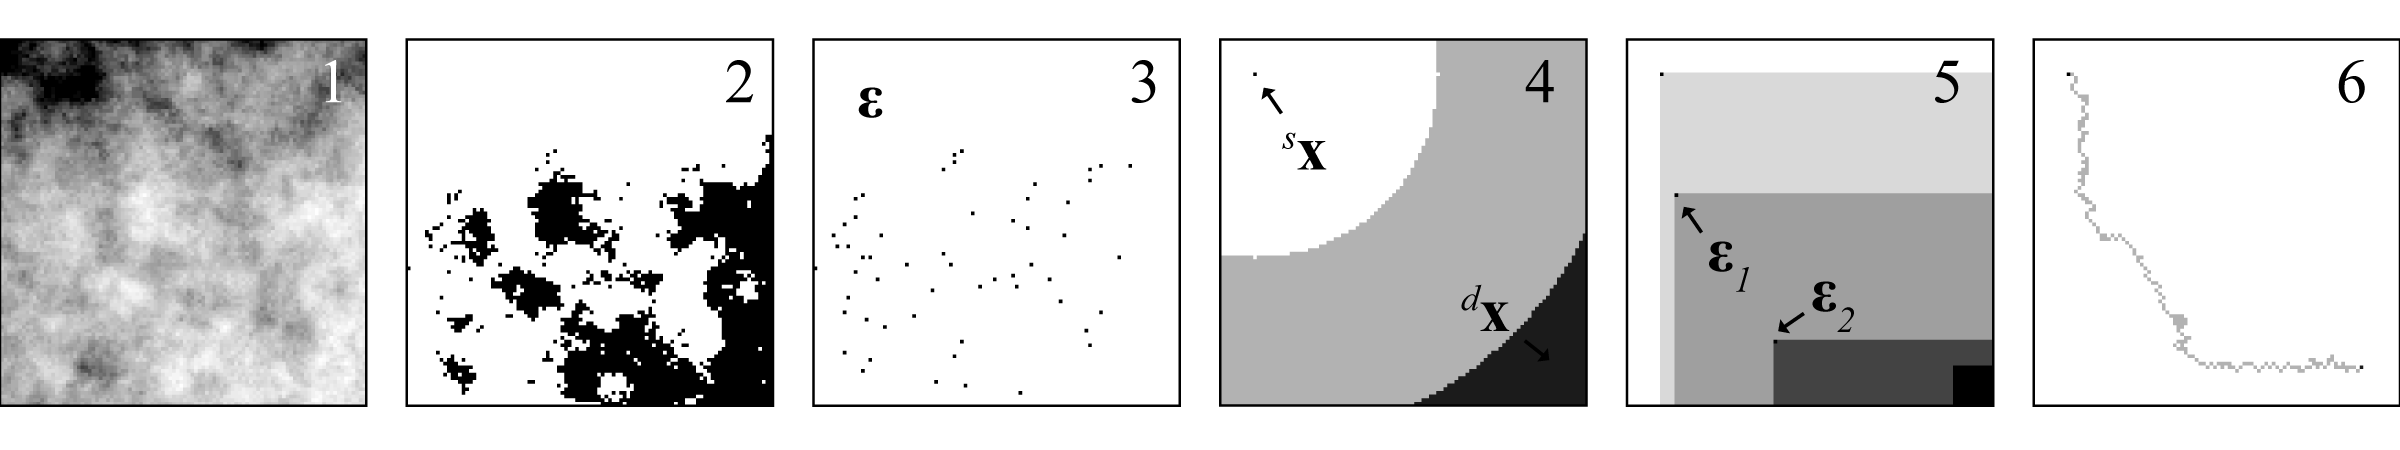
\includegraphics[width=5.5in]{figures/multi-part-pseudo-random-walk-example.png}
            \caption[Conceptual Illustration of a Multi-Part Pseudo-Random Walk]{Conceptual Illustration of a Multi-Part Pseudo-Random Walk}
            \label{fig:multi-part-pseudo-random-walk-example}
            \end{figure}
            
The multi-part walk process is described by the sequence of panels moving from left to right within Figure 5. [1] The process begins with the far left panel which plots the value of the objective variables within the a square 2-D search domain. [2] The first step is to create a binary mask of feasible nodes by selecting objective surface values less than some arbitrary threshold. [3] The next step involves determining the cell indices for the set of centroid nodes $\epsilon$ computed from the connected components within this binary mask. [4] After this, these centroids are assigned rankings on the basis of their inclusion in bins of progressive Euclidean distance from the source location. [5] Next, the procedure requires the iterative selection of centroids $\epsilon_1, \epsilon_2$, one from each successive distance bin, until the bin containing the destination location is reached. The centroid selection process can be unstructured, random within each bin, or structured (as shown), where the centroids considered eligible for selection each iteration is restricted to those orientated positively in the direction of the destination. [6] Finally, the source is connected to the destination a series of pseudo-random walks constructed for sequential pairs of the selected centroids.
            
\section{Initializing Problems with Concave Decision Spaces}
            
Another circumstance which has the potential to dramatically effect the performance of the pseudo-random walk procedure are problem specifications in which all or a portion of the Euclidean path connecting the source to the destination falls outside the feasible area of the search domain. Such a circumstance can be described as a concave problem, as the source and destination locations are not convex to one another within the boundaries of the decision space $\Omega$. Concave problem statements have the potential to create a situation where at each iteration $n$ of the pseudo-random walk process large values of $u$ must be attained before the covariance term is relaxed enough to allow for the sampling process to generate a $\Delta\textbf{x}_u$ that is contained within the valid set $\textbf{V}_n$. In a worst case scenario, the entire runtime improvement associated with the pseudo-random walk based population initialization procedure might be lost.

An approach which has been developed to address such cases is the so called concave multi-part pseudo random walk. It is similar to the standard multi-part walk in that the final walk is composed of a collection of pseudo-random walk sections. However, it differs from the standard walk procedure in that rather than partitioning the space on the basis of distance bands, it iteratively divides the decision space into a series of convex subregions. Here again, these convex sub region contain the centroids associated with connected regions of low objective variable values. The procedure is illustrated conceptually by the sequence of panels contained in Figure 6.
            
            \begin{figure}[!h]
            \centering
            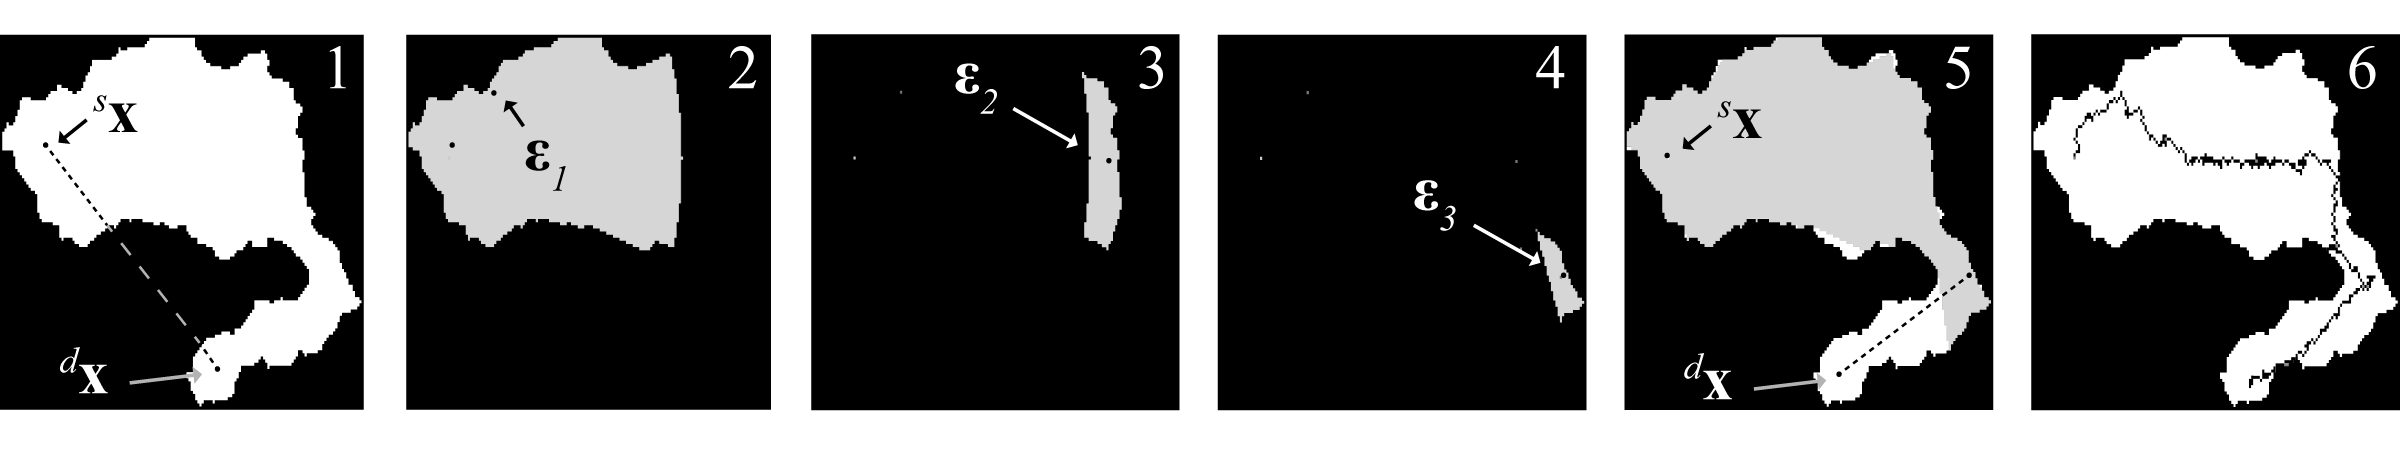
\includegraphics[width=5.5in]{figures/convex-multi-part-pseudo-random-walk-example.png}
            \caption[Conceptual Illustration of a Convex Multi-Part Pseudo-Random Walk]{Conceptual Illustration of a Convex Multi-Part Pseudo-Random Walk}
            \label{fig:convex-multi-part-pseudo-random-walk-example}
            \end{figure}
            
The concave multi-part walk process is described by the sequence of panels moving from left to right within Figure 6. [1] In the first panel, on the far left, we can see a problem that has been posed in such a way that the Euclidean path connecting the source to the destination is not feasible as it exits the boundaries of the search domain. [2]  For brevity, the two subsequent steps are not shown as they are identical to steps 2-3 in the standard multi-part pseudo random walk procedure. These omitted steps involve the generation of candidate centroids from the connected components within the objective surface. The next illustrated step, shown in the panel second from left, involves computing all of the row column indices that are convex to the source location.Within this convex region a the first centroid $\epsilon_1$ is selected. Here again, the process can be unstructured, where the entire convex region is searched, or structured  (as shown), where the initial convex region is restricted to some maximum distance from the source. [3-4] From here, additional non-overlapping convex subregions are computed and candidate centroids iteratively selected from within them. [5] The centroid selection process concludes when the current convex region contains the destination location. [6] Finally, the source is connected to the destination, as in the simple multi-part case, by a series of pseudo-random walks constructed for sequential pairs of the selected centroids.

\section{Measuring Initialization Performance}
    
The stochastic processes inherent to the pseudo-random walk procedure, as well as to many other components of the MOGADOR algorithm, make it difficult to analytically derive performance characteristics. As a consequence, with MOGADOR, as with many other GAs, features such as runtime performance must be evaluated through empirical observation. The following sections introduce the results obtained from several such empirical investigations related to the performance of the pseudo-random walk based population initialization procedure for the MOGADOR algorithm. For reference, all computations were performed using a desktop class hardware possessing a 2.3 GHz Intel Quad Core i7 processor (2nd Gen.) with 16 GB of system RAM.
            
The first of these investigations seeks to understand the role of the fixed parameter $q$, embedded in the pseudo-random walk covariance generator function, in determining the structural characteristics of output populations. In order to study this issue, a synthetic problem statement was created. This problem statement involves a square search domain of 100 nodes on a side – resulting in a total problem size of $\boldsymbol\Omega = 10,000$ nodes. The value of the estimated objective function $\hat{O}_w$ used to evaluate fitness was set as constant for all of the nodes in the search domain. In this way, the objective score is roughly equivalent to individual walk length in Euclidean space. Using this problem statement, twenty seed populations, all containing $m = 100$ individuals, were generated  using monotonically increasing values of $q$ beginning with $q = 0.5$ and concluding with $q = 10$. For each the generated populations, the average objective scores for all individuals as well as the standard deviation of the objective scores among individuals were evaluated. The results of this empirical investigation are presented in Figure 7.
            
            \begin{figure}[Observing the Role of the Fixed Parameter $q$ in Determining Individual Path Randomness]
            \centering
            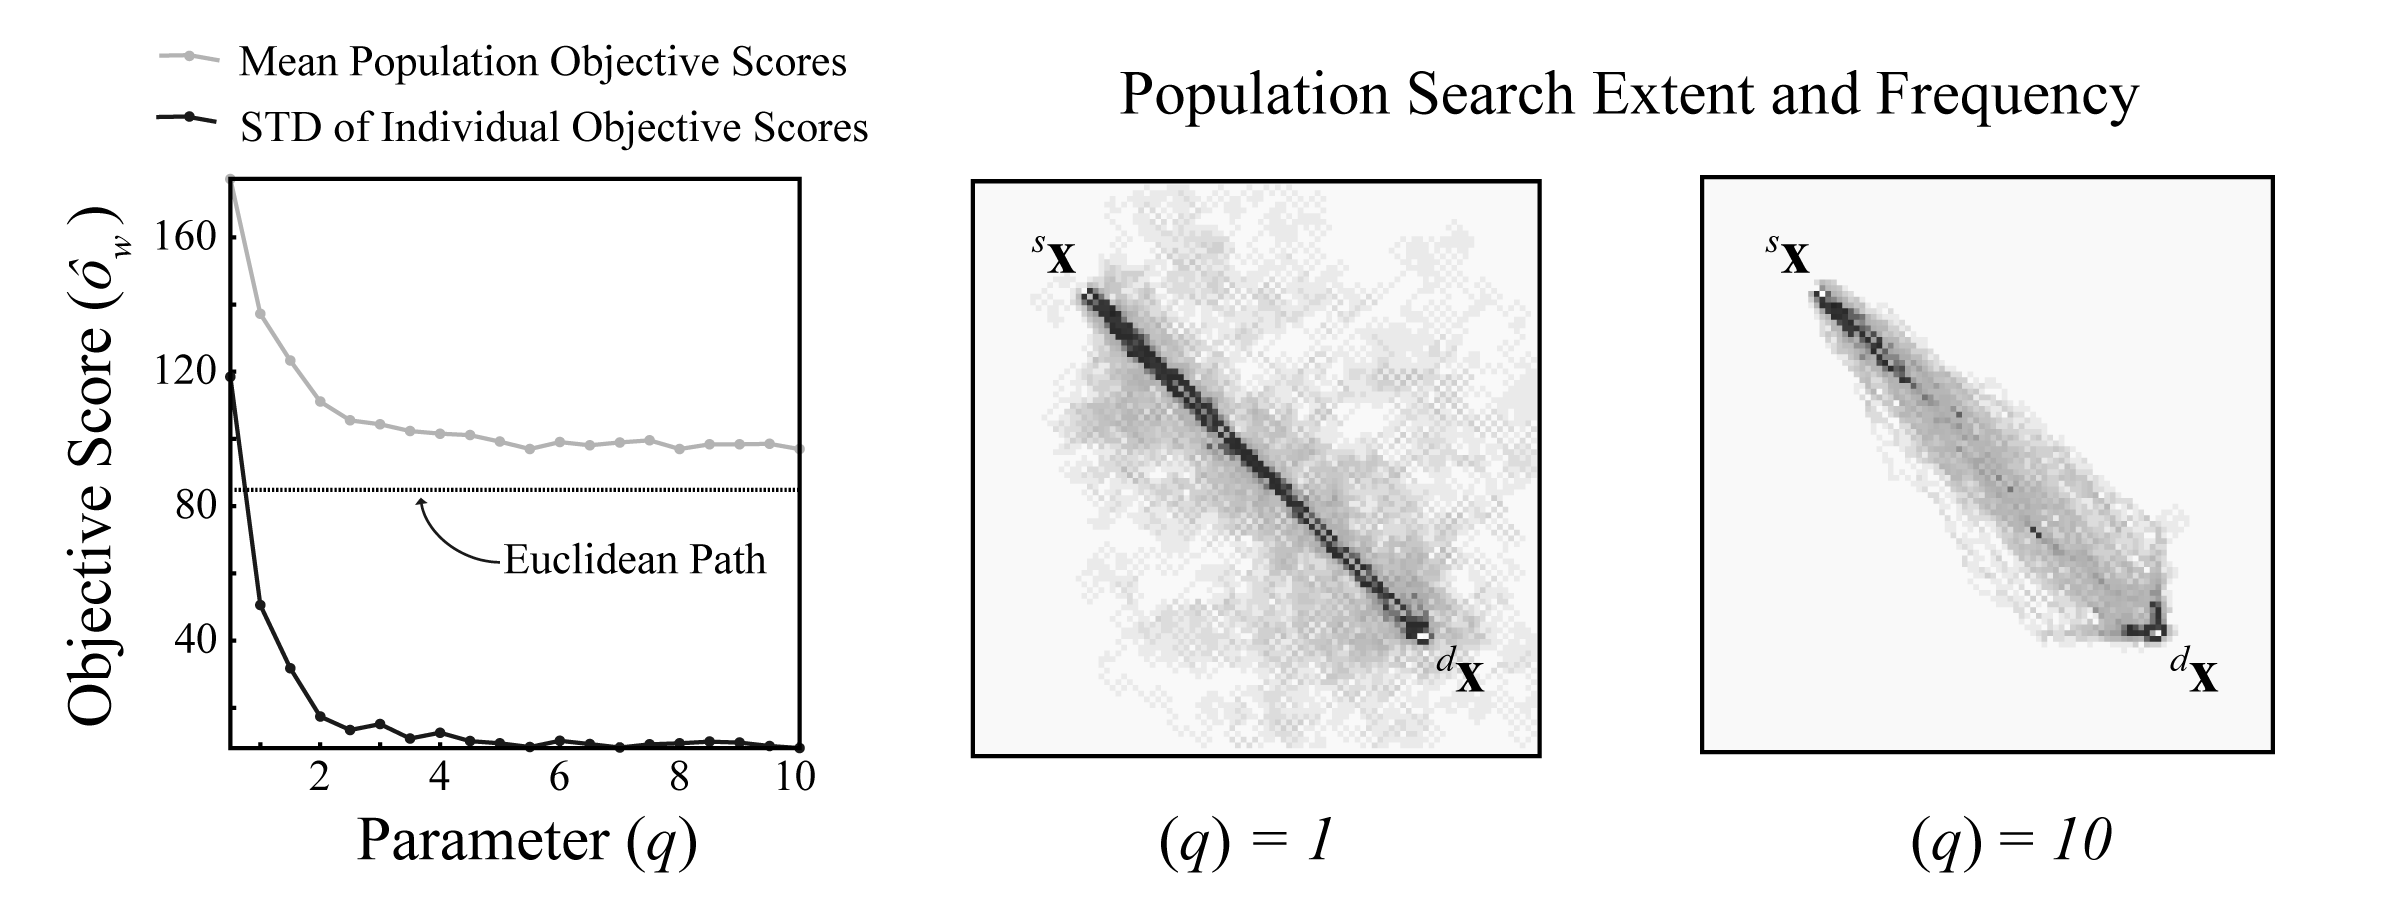
\includegraphics[width=5.5in]{figures/path-randomness-study.png}
            \caption[Observing the Role of the Fixed Parameter $q$ in Determining Individual Path Randomness]{Observing the Role of the Fixed Parameter $q$ in Determining Path Randomness}
            \label{fig:path-randomness}
            \end{figure}
            
As Figure 7 illustrates, increasing the value of the fixed parameter $q$ causes the individuals within the a population to more closely approximate the Euclidean shortest path between the source and destination. Similarly, relaxation of this parameter results in an increase in the perceived randomness among the individual walks within a population. These attributes can be clearly observed in the two images to the right of Figure 7 which show the frequency with which every node within the search domain has been visited by any individual within two populations generated from different values of $q$.
            
Another issue warranting empirical investigation is the relationship between runtime performance of the proposed initialization procedure and problem size. In order to study this issue a series of ten synthetic problem statements were constructed with near identical structural components; differing from on another only in terms of problem size. In each of these problem statements the source location was positioned one fifth of the way down and to the right from the top left of the search domain and, likewise, the destination location was positioned a constant one fifth of the way up from the bottom right corner of the search domain. For all of the different populations generated, the value of the fixed parameter $q$ was set relatively high $q = 10$ to reduce computational effort.
            
            \begin{figure}[Observing the Role of Problem Size on Initialization Runtime]
            \centering
            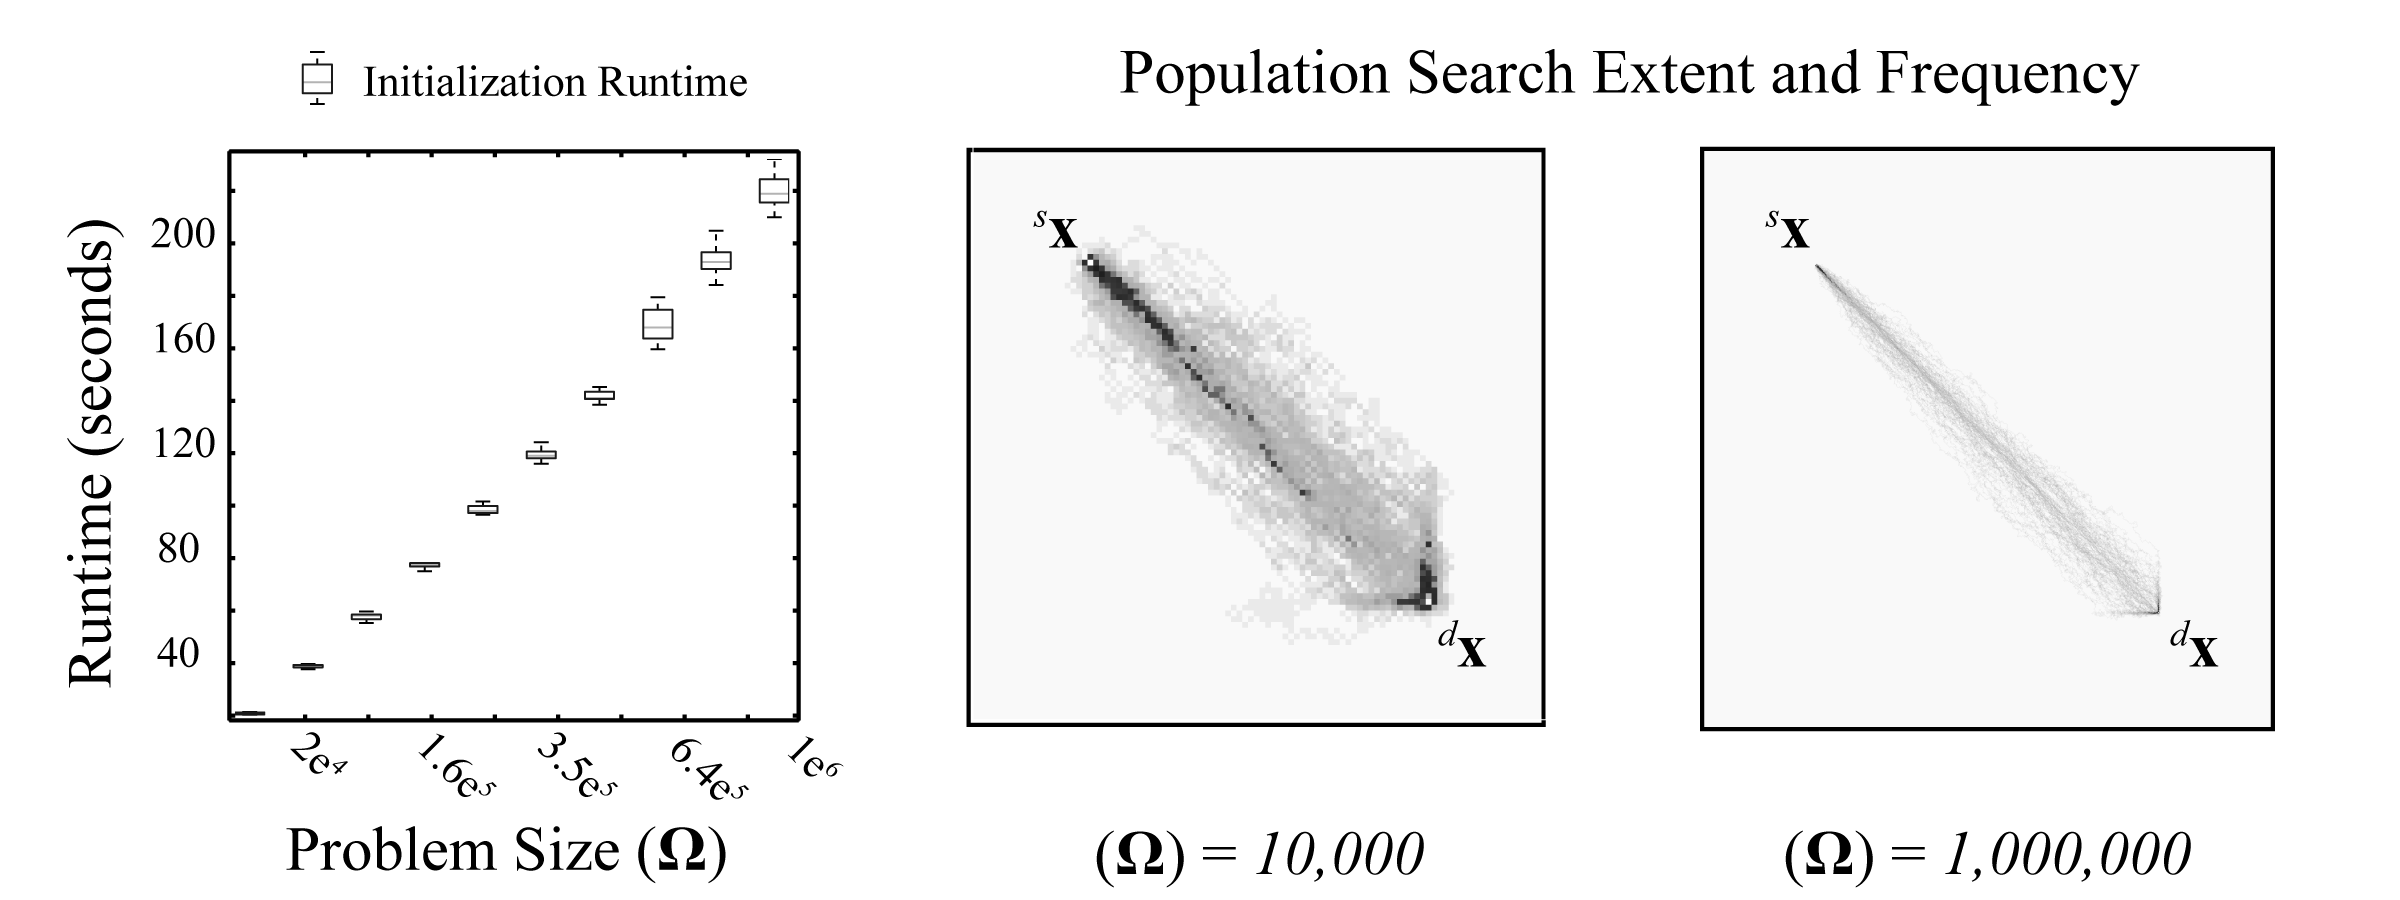
\includegraphics[width=5.5in]{figures/problem-size-study.png}
            \caption[Observing the Role of Problem Size on Initialization Runtime]{Observing the Role of Problem Size on Initialization Runtime}
            \label{fig:problem-size}
            \end{figure}
            
The plot to the left of Figure 8 illustrates the the distributional properties of the runtimes required to generate ten replicate populations for the ten problem statements of progressively increasing size – resulting in a total of $g = 100$ unique populations, each comprised of $m = 100$ individuals. Such repeated simulation is necessary as the proposed initialization routine is based upon a stochastic sampling process which can and will deliver variable runtimes for the repeated applications to the same problem context. One feature of note in this plot is the roughly linear relationship between the mean runtime and problem size for this type of pseudo-random walk based approach to the problem initialization procedure for the range of problem sizes considered. The two images to the right illustrate the effective search extent and frequency for the smallest and the largest populations generated during this investigation.
            
One of the considerations previously discussed related to the initialization of the MOGADOR algorithm in the context of large problem statements was the need to ensure sufficient diversity within the seed population for the search process to be conducted at the global level. This problem is clearly evident in the population search extent and frequency image contained on the far right of Figure 8.  In this example, the population clearly fails to explore a sufficiently large portion of the decision space to be considered as a form of global search. The solution which was previously proposed to this problem involved generating so called multi-part pseudo-random walks. The subsequent investigation therefore, compares the statistical characteristics of a set of populations generated from standard pseudo-random walk to another set of population generated from multi-part pseudo random walks. The results of this investigation are provided in Figure 9.
            
            \begin{figure}[Observing the Characteristics of Multi-Part Pseudo-Random Walks]
            \centering
            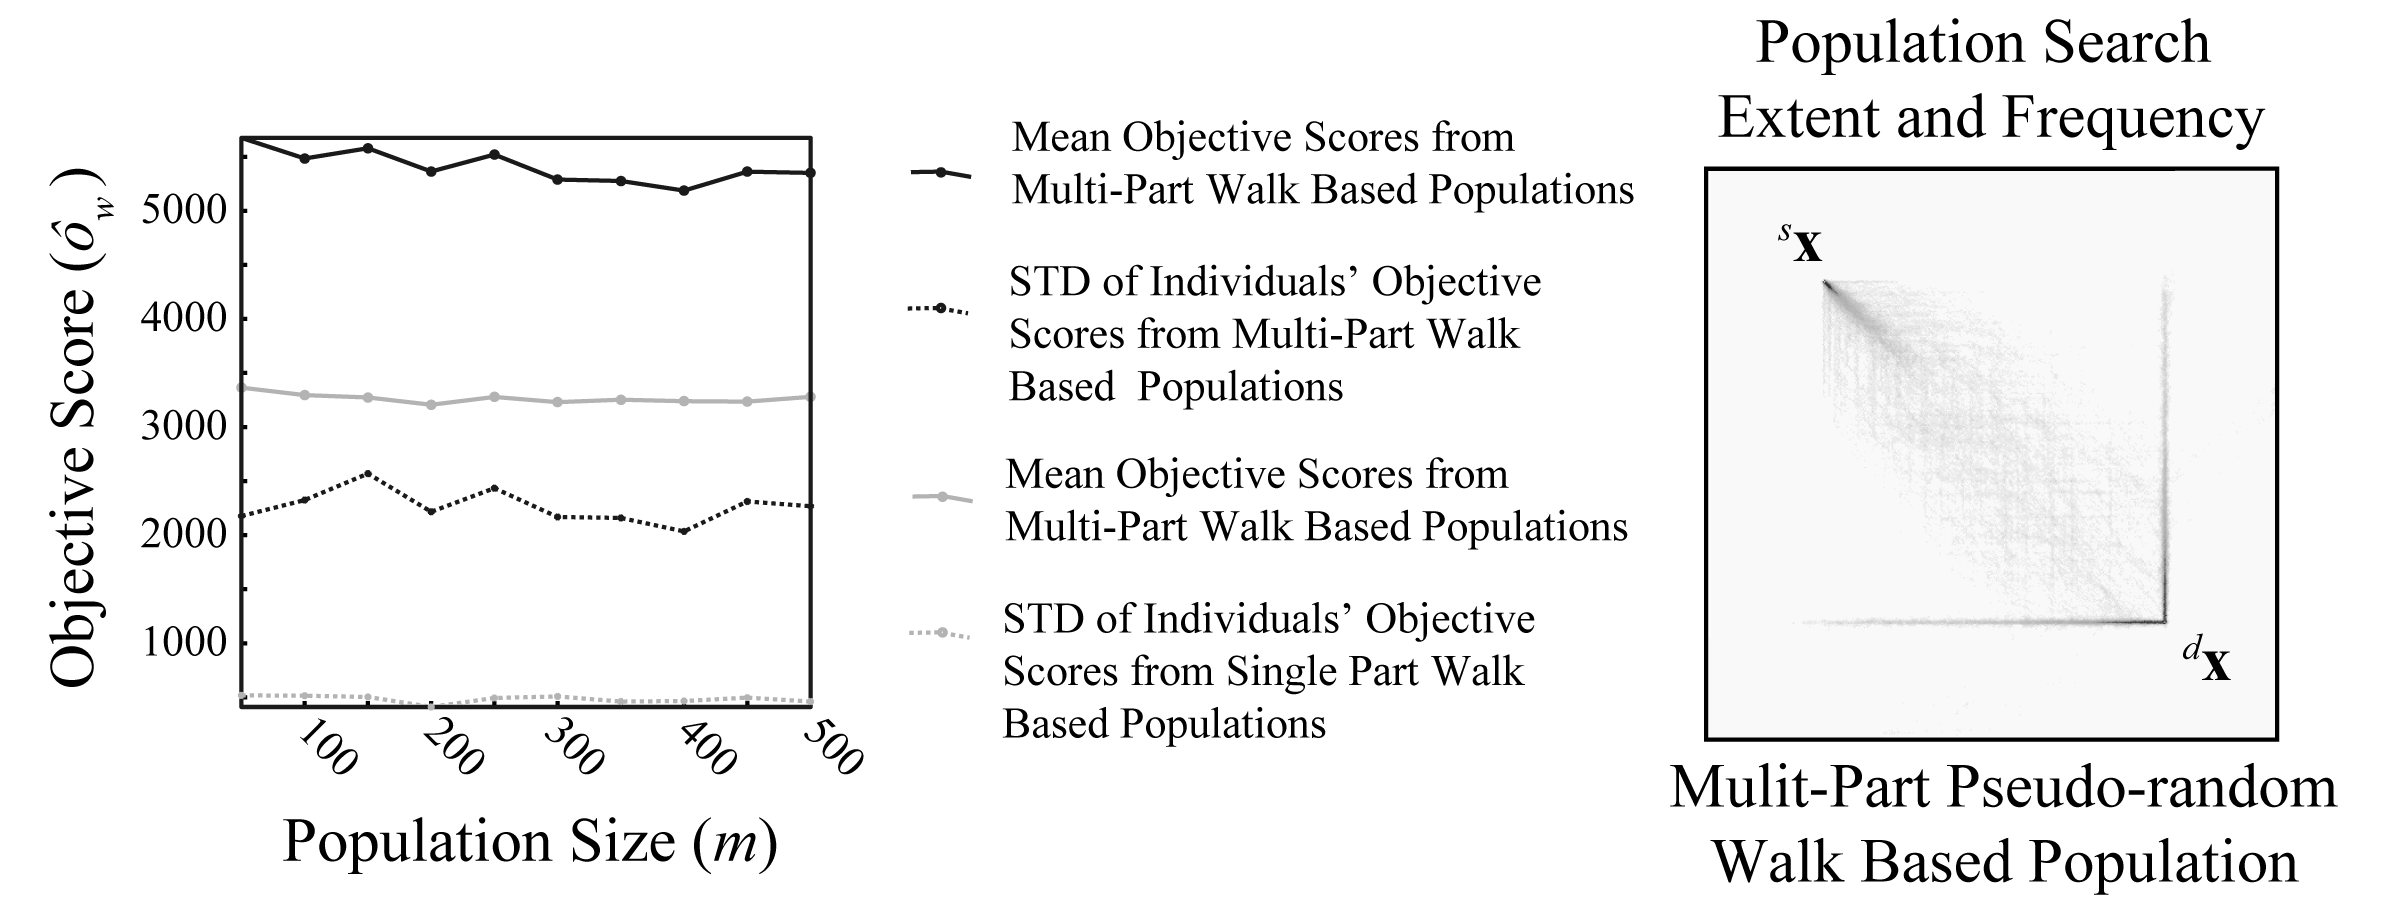
\includegraphics[width=5.5in]{figures/multi-part-walk-study.png}
            \caption[Observing the Characteristics of Multi-Part Pseudo-Random Walks]{Observing the Characteristics of Multi-Part Pseudo-Random Walks}
            \label{fig:multi-part-walk-study}
            \end{figure}
            
The runtime reductions which can be achieved from the use of the multi-part pseudo random walk procedure will principally occur in the context of relatively high value settings for the fixed parameter $q$. This is because while the various component segments of a multi-part walk may not deviate significantly from the Euclidean shortest path however, the randomized connection of multiple such segments produces composite individuals that are significantly more diverse.
            
\section{MOGADOR Algorithm Outputs}
